\section{Partial Derivatives}
\label{sec:derivatives}

Now that you have some familiarity with functions of two variables, it's time to start applying calculus to help us solve problems with them. In Chapter \ref{ch:derivatives}, we learned about the derivative\index{Derivative} for functions of two variables. Derivatives told us about the shape of the function, and let us find local max and min – we want to be able to do the same thing with a function of two variables.

First let's think. Imagine a surface, the graph of a function of two variables. Imagine that the surface is smooth and has some hills and some valleys. Concentrate on one point on your surface. What do we want the derivative to tell us? It ought to tell us how quickly the height of the surface changes as we move… Wait, which direction do we want to move? This is the reason that derivatives are more complicated for functions of several variables – there are so many (in fact, infinitely many) directions we could move from any point.

It turns out that our idea of fixing one variable and watching what happens to the function as the other changes is the key to extending the idea of derivatives to more than one variable.

\begin{definition}[Partial Derivatives]
Suppose that $z=f(x,y)$ is a function of two variables.
\begin{itemize}
  \item The {\bf partial derivative}\index{Partial derivative}\index{Derivative!partial} of $f$ {\bf with respect to} $x$ is the derivative of the function $f(x,y)$ where we think of $x$ as the only variable and act as if $y$ is a constant.
  \item The partial derivative of $f$ with respect to $y$ is the derivative of the function $f(x,y)$ where we think of $y$ as the only variable and act as if x is a constant.
\end{itemize}
The ``with respect to $x$'' or ``with respect to $y$'' part is really important -- you have to know and tell which variable you are thinking of as THE variable.

{\bf Geometrically}, the partial derivative with respect to $x$ gives the slope of the curve as you travel along a cross-section, a curve on the surface parallel to the $x$-axis. The partial derivative with respect to $y$ gives the slope of the cross-section parallel to the $y$-axis.

{\bf Notation for the Partial Derivative}
The partial derivative of $z=f(x,y)$ with respect to $x$ is written as
$$f_x(x,y)$$
or simply
$$f_x \quad\mbox{or}\quad z_x \enspace .$$
The {\bf Leibniz notation}\index{Leibniz notation} is
$$\frac{\partial f}{\partial x} \quad \mbox{or} \quad \frac{\partial z}{\partial x} \enspace .$$
We use an adaptation of the $\dfrac{\partial z}{\partial x}$ notation to mean find the partial derivative of $f(x,y)$ with respect to $x$:
$$\frac{\partial}{\partial x}f(x,y)=\frac{\partial f}{\partial x} \enspace .$$

{\bf Estimate a partial derivative from a table or contour diagram}
The partial derivative with respect to $x$ can be approximated by looking at an average rate of change, or the slope of a secant line, over a very tiny interval in the $x$-direction (holding $y$ constant). The tinier the interval, the closer this is to the true partial derivative.

{\bf Compute a partial derivative from a formula}
If $f(x,y)$ is given as a formula, you can find the partial derivative with respect to $x$ algebraically by taking the ordinary derivative thinking of $x$ as the only variable (and treating $y$ as an ordinary number).

Of course, everything here works the same way if we're trying to find the partial derivative with respect to $y$ -- just think of $y$ as your only variable and act as if $x$ is constant.

The idea of a partial derivative works perfectly well for a function of several variables: you focus on one variable to be THE variable and act as if all the other variables are constants.
\end{definition}
\begin{example}
Figure \ref{fig:4-2-ex1} shows a contour diagram for a function $g(x,y)$.

\begin{figure}[!ht]
  \centering
    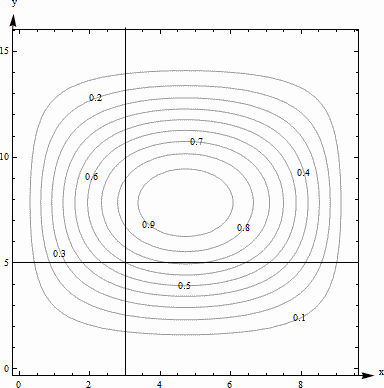
\includegraphics[width=0.4\textwidth]{img/chap4/image026.png}
    \caption{$z = g(x, y)$}
    \label{fig:4-2-ex1}
\end{figure}

Use the diagram to answer the following questions:
  \begin{enumerate}[label=(\alph*)]
    \item Estimate $g_x(3,5)$ and $g_y(3,5)$.

    \begin{solution} $g_x(3,5)$ means we're thinking of $x$ as the only variable, so we'll hold $y$ fixed at $y=5$. That means we’ll be looking along the horizontal line $y=5$. To estimate $g_x$, we need two function values. $(3, 5)$ lies on the contour line, so we know that $g(3,5)=0.6$. The next point as we move to the right is $g(4.2,5)=0.7$.

    Now we can find the average rate of change:
    \begin{align*}
    \mbox{Average rate of change} &= \frac{\mbox{change in output}}{\mbox{change in input}}\\
    &= \frac{\Delta g}{\Delta x}\\
    &= \frac{0.7-0.6}{4.2-3}\\
    &= \frac{1}{12}\approx   0.083
    \end{align*}
    We can do the same thing by going to the next point we can read to the left, which is $g(2.4,5)=0.5$. Then the average rate of change is
    $$ \frac{\Delta g}{\Delta x} = \frac{0.5-0.6}{2.4-3}=\frac{1}{6} \approx   0.167 \enspace .$$
    Either of these would be a fine estimate of $g_x(3,5)$ given the information we have, or we could take their average. We can estimate that $g_x(3,5)\approx   0.125$.

    Estimate $g_y(3,5)$ the same way, but moving on the vertical line. Using the next point up, we get the average rate of change is
    $$\frac{\Delta g}{\Delta y} = \frac{0.7-0.6}{5.8-5}=\frac{1}{8}=0.125 \enspace .$$
    Using the next point down, we get
    $$ \frac{\Delta g}{\Delta y}=\frac{0.5-0.6}{4.5-5}=\frac{1}{5}=0.2 \enspace .$$
    Taking their average, we estimate $g_y(3,5)\approx   0.1625$.
    \end{solution}
    \item Where on this diagram is $g_x$ greatest? Where is $g_y$ greatest?

    \begin{solution}
    $g_x$ means $x$ is our only variable, and we're thinking of $y$ as a constant. So we're thinking about moving across the diagram on horizontal lines. $g_x$ will be greatest when the contour lines are closest together, i.e., when the surface is steepest – then the denominator in $\dfrac{\Delta g}{\Delta x}$ will be small, so $\dfrac{\Delta g}{\Delta x}$ will be big. Scanning the graph in Figure \ref{fig:4-2-ex1}, we can see that the contour lines are closest together when we head to the left or to the right from about $(0.5, 8)$ and $(9, 8)$. So $g_x$ is greatest at about $(0.5, 8)$ and $(9, 8)$. For $g_y$, we want to look at vertical lines. $g_y$ is greatest at about $(5, 3.8)$ and $(5, 12)$.
    \end{solution}
  \end{enumerate}
\end{example}

\begin{example}
Cold temperatures feel colder when the wind is blowing. Windchill, $W$, is the perceived temperature, and it depends on both the actual temperature, $T$, and the wind speed, $V$, so $W = W(T, V)$ is a function of two variables! You can read more about windchill at \url{http://www.nws.noaa.gov/om/windchill/}. The table in Figure \ref{fig:4-2-windchill} shows the perceived temperature for various temperatures and windspeeds.

\begin{figure}[!ht]
  \centering
    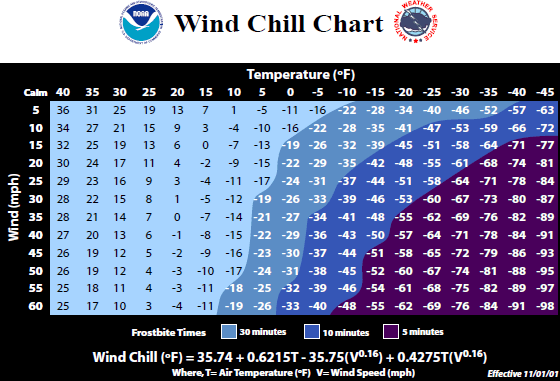
\includegraphics[width=0.4\textwidth]{img/chap4/image045.png}
    \caption{Windchill table, National Weather Service}
    \label{fig:4-2-windchill}
\end{figure}

Note that they also include the formula, but for this example we'll use the information in the table.
\begin{enumerate}
  \item What is the perceived temperature when the actual temperature is 25$^{\circ}$F and the wind is blowing at 15 miles per hour?

  \begin{solution}
    Reading the table, we see that the perceived temperature is $W(25, 15) = 13^{\circ}$F.
  \end{solution}
  \item Suppose the actual temperature is 25$^{\circ}$F. Use information from Table \ref{fig:4-2-windchill} to describe how the perceived temperature would change if the wind speed increased from 15 miles per hour?

  \begin{solution}
    This is a question about a partial derivative. We’re holding the temperature fixed at $T = 25^{\circ}$F, and asking what happens as wind speed ($V$) increases from 15 miles per hour. We’re thinking of $V$ as the only variable, so we want to estimate $W_V(25, 15)$. We'll find the average rate of change by looking in the column where $T=25$ and letting $V$ increase, and use that to approximate the partial derivative.
    $$W_V \approx  \frac{\Delta W}{\Delta V} = \frac{11-13}{20-15} = -0.4 \enspace .$$
    What are the units? $W$ is measured in $^{\circ}$F and $V$ is measured in mph, so the units here are $^{\circ}$F/mph. And that lets us describe what happens. The perceived temperature would decrease by about 0.4$^{\circ}$F for each mph increase in wind speed.
\end{solution}
\end{enumerate}
\end{example}

\begin{example}
Find $f_x$ and $f_y$ at the points $(0, 0)$ and $(1, 1)$ if $f(x,y)=x^2-4xy+4y^2$.

\begin{solution}
  To find $f_x$, take the ordinary derivative of $f$ with respect to $x$, acting as if $y$ is constant:
$$f_x(x,y)=2x-4y \enspace .$$
Note that the derivative of the term $4y^2$, with respect to $x$, is $0$ because it's a constant (as far as $x$ is concerned).

Similarly,
$$f_y(x,y)=-4x+8y \enspace .$$
Now we can evaluate these at the points:

$f_x(0,0)=0$ and $f_y(0,0)=0$; this tells us that the cross sections parallel to the $x$ and $y$-axes are both flat at $(0,0)$.

$f_x(1,1)=-2$ and $f_y(1,1)=4$; this tells us that above the point $(1, 1)$, the surface decreases if we move to more positive $x$ values and increases if we move to more positive $y$ values.
\end{solution}\end{example}

\begin{example}
  \label{ex:4-partials}
Find $\dfrac{\partial f}{\partial x}$ and $\dfrac{\partial f}{\partial y}$ if $f(x,y)=\frac{e^{x+y}}{y^3+y} + y\ln(y)$.

\begin{solution}
  $\dfrac{\partial f}{\partial x}$ means $x$ is our only variable, we're thinking of $y$ as a constant. Then we'll just find the ordinary derivative. From the point of view of $x$, this is an exponential function, divided by a constant, with a constant added. The constant pulls out in front, the derivative of the exponential function is the same thing, and we need to use the chain rule, so we multiply by the derivative of that exponent (which is just 1):
$$\frac{\partial f}{\partial x} = \frac{1}{y^3+y}\cdot e^{x+y} \enspace .$$
$\dfrac{\partial f}{\partial y}$ means that we're thinking of $y$ as the variable, acting as if $x$ is constant. From $y$'s point of view, $f$ is a quotient plus a product, so we'll need the quotient rule and the product rule:
\begin{align*}
\frac{\partial f}{\partial y} &= \frac{( )( )-( )( )}{( )^2}+( )( )+( )( ) \\
 &= \frac{\left(e^{x+y}(1)\right)(y^3+y)-\left(e^{x+y}\right)(3y^2+1)}{(y^3+y)^2}+(1)(\ln(y))+(y)\left(\frac{1}{y}\right)
\end{align*}
\end{solution}\end{example}

\begin{example}
Find $f_z$ if $f(x,y,z,w)=35x^2w - \frac{1}{z}+yz^2$.

\begin{solution}
$f_z$ means we act as if $z$ is our only variable, so we'll act as if all the other variables ($x$, $y$, and $w$) are constants and take the ordinary derivative:
$$f_z(x,y,z,w) = \frac{1}{z^2} + 2yz \enspace .$$
\end{solution}\end{example}

\subsection{Using Partial Derivatives to Estimate Function Values}
We can use the partial derivatives to estimate values of a function. The geometry is similar to the tangent line approximation in one variable. Recall the one-variable case: if $x$ is close enough to a known point $a$, then
$$f(x)\approx   f(a)+f'(a)(x-a) \enspace .$$
In two variables, we do the same thing in both directions at once:

\begin{theorem}[Approximating Function Values with Partial Derivatives]
To approximate the value of $f(x,y)$ where the point $(x, y)$ is near a point $(a,b)$, especially when the exact values of $f(a,b)$, $f_x(a, b)$, and $f_y(a, b)$ exist and are easy to compute, then:
$$f(x,y)\approx   f(a,b)+f_x(a,b)(x-a)+f_y(a,b)(y-b) \enspace .$$
Notice that the total change in $f$ is being approximated by adding the approximate changes coming from the $x$ and $y$ directions. Another way to look at the same formula is :
$$ \Delta f\approx   f_x\Delta x+f_y\Delta y \enspace . $$
\end{theorem}
How close is close? It depends on the shape of the graph of $f$. In general, the closer the better.

\begin{example}
Use partial derivatives to estimate the value of $f(x,y)=x^2-4xy+4y^2$ at the point $(0.9, 1.1)$.

\begin{solution}
  Note that the point $(0.9, 1.1)$ is close to an easy point, $(1, 1)$. In fact, we already worked out the partial derivatives at $(1, 1)$: $f_x(x,y)=2x-4y$ so $f_x(1,1)=-2$, and $f_y(x,y)=-4x+8y$ so $f_y(1,1)=4$. We also know that $f(1,1)=1$.

So,
$$f(0.9,1.1)\approx   1-2(-0.1)+4(0.1)=1.6 \enspace .$$
Note that in this example it would have been possible to simply compute the exact answer:
$$f(0.9,1.1)=(0.9)2-4(0.9)(1.1)+4(1.1)2=1.69 \enspace .$$
Our estimate is not perfect, but it's pretty close.
\end{solution}\end{example}

\begin{example}
Figure \ref{fig:4-2-ex7} shows a contour diagram for a function $g(x,y)$. Use partial derivatives to estimate the value of $g(3.2,4.7)$.

\begin{figure}[!ht]
  \centering
    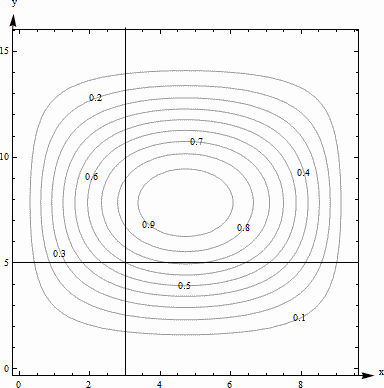
\includegraphics[width=0.4\textwidth]{img/chap4/image026.png}
    \caption{$z = g(x, y)$}
    \label{fig:4-2-ex7}
\end{figure}
\begin{solution}
  This is the same diagram from before, so we already estimated the value of the function and the partial derivatives at the nearby point $(3,5)$. $g(3,5)$ is 0.6, our estimate of $g_x(3,5)\approx   0.125$, and our estimate of $g_y(3,5)\approx   0.1625$. So
$$g(3.2,4.7)\approx   0.6+(0.125)(0.2)+(0.1625)(-0.3)=0.57625 \enspace .$$
Note that in this example we have no way to know how close our estimate is to the actual value.
\end{solution}\end{example}

% Application: Option pricing and "the Greeks."
